% =============================================================
%  Test document: TikZ single-line diagram of a cable link
%  Uses the shared American Terawatt report style.
%  Compile:  pdflatex transmission-line.tex   (run twice)
% =============================================================
\documentclass[11pt,a4paper]{article}

% Shared style lives in the repo-level template folder
\usepackage[corporate]{../../template/attemplate}

% TikZ libraries used by the figure
\usetikzlibrary{arrows.meta,calc}

% ---- Report metadata ----------------------------------------
\reporttitle{Cable Link Single-Line Diagram}
\reportsubtitle{TikZ rendering of the sending-end / receiving-end transmission model}
\atEyebrow{Template test}
\atAbstract{Test document for the shared report template. It compiles a
TikZ rendering of the single-line diagram of a cable transmission link
(source, disconnectors, cable of length $L_{\mathrm{cable}}$ and load
impedance $Z_{L}$) with the sending-end and receiving-end voltages,
currents and power flows.}
\reportauthor{Eugen Starschich}
\reportdocnumber{ATW-TST-TIKZ-001}
\reportrevision{0.1}
\reportstatus{Draft}
\reportdate{\today}
\reportconfidentiality{Internal}

\begin{document}

\makecover

\revisionhistory{
  \revrow{0.1}{Sep. 18, 2026}{Eugen Starschich}{Initial document}
}

\clearpage

% ---- Body ---------------------------------------------------
\section{Transmission model}

Figure~\ref{fig:transmission-line} shows the single-line representation of
a cable transmission link between a sending end $S$ and a receiving end
$R$. The sending-end source feeds the cable through a disconnector; at the
receiving end a second disconnector connects the cable to the load
impedance $Z_{L}$. The voltages $U_{S}$ and $U_{R}$ are measured against
ground at the two cable ends, the currents $I_{S}$ and $I_{R}$ are counted
positive in the direction from $S$ to $R$, and $P_{S}, Q_{S}$ and
$P_{R}, Q_{R}$ denote the active and reactive power entering and leaving
the cable of length $L_{\mathrm{cable}}$.

\begin{figure}[!ht]
  \centering
  \resizebox{\linewidth}{!}{% -------------------------------------------------------------
%  Single-line diagram of a cable transmission link
%  TikZ rendering of image9.pdf (sending end S, cable, receiving
%  end R with load impedance Z_L). Include with \input{...} inside
%  a figure environment; tikz is loaded by the shared template.
%  Requires: \usetikzlibrary{arrows.meta}
% -------------------------------------------------------------
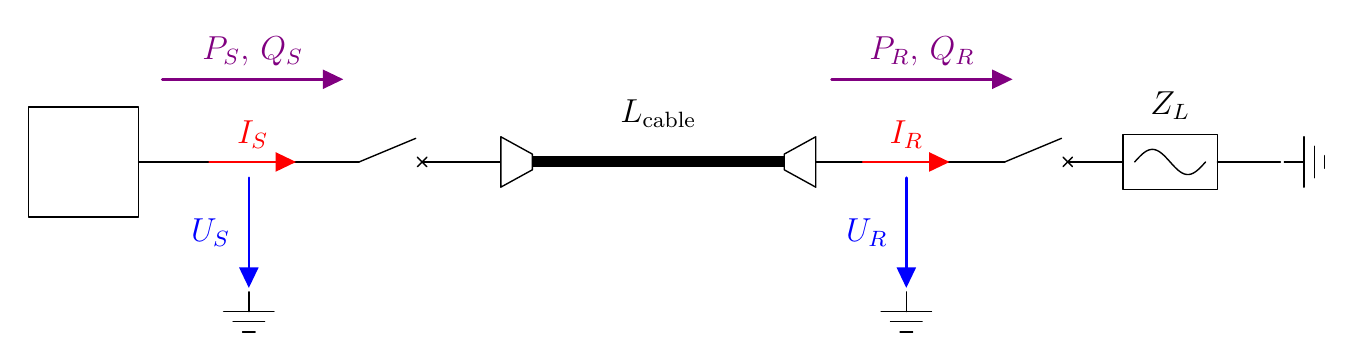
\begin{tikzpicture}[
  line cap=round, line join=round,
  wire/.style={draw=black, line width=0.5pt},
  cable/.style={draw=black, line width=4pt, line cap=butt},
  current/.style={draw=red,    line width=0.9pt, -{Triangle[length=2.6mm,width=2.4mm]}},
  voltage/.style={draw=blue,   line width=0.9pt, -{Triangle[length=2.6mm,width=2.4mm]}},
  power/.style={draw=violet,   line width=0.9pt, -{Triangle[length=2.6mm,width=2.4mm]}},
  lbl/.style={font=\sffamily\large},
  % ground symbol: three bars of decreasing width, anchored at the top
  pics/ground/.style={code={
      \draw[wire] (0,0) -- (0,-0.25);
      \draw[wire] (-0.32,-0.25) -- (0.32,-0.25);
      \draw[wire] (-0.20,-0.38) -- (0.20,-0.38);
      \draw[wire] (-0.08,-0.51) -- (0.08,-0.51);
  }},
  % open disconnector: contacts at (0,0) and (0.8,0)
  pics/switch/.style={code={
      \draw[wire] (0,0) -- (0.72,0.30);
      \draw[wire] (0.74,-0.06) -- (0.86,0.06);
      \draw[wire] (0.74,0.06) -- (0.86,-0.06);
      \draw[wire] (0.8,0) -- (0.95,0);
  }},
]
  % ---- sending end -------------------------------------------
  \draw[wire] (0,-0.7) rectangle (1.4,0.7);          % source / converter block
  \draw[wire] (1.4,0) -- (4.2,0);
  \draw[current] (2.3,0) -- (3.4,0) node[midway, above=1pt, lbl, red] {$I_{S}$};
  \draw[voltage] (2.8,-0.2) -- (2.8,-1.6) node[midway, left=3pt, lbl, blue] {$U_{S}$};
  \pic[blue] at (2.8,-1.65) {ground};
  \draw[power] (1.7,1.05) -- (4.0,1.05) node[midway, above=1pt, lbl, violet] {$P_{S},\,Q_{S}$};

  % ---- sending-end disconnector ------------------------------
  \pic at (4.2,0) {switch};
  \draw[wire] (5.15,0) -- (6.0,0);

  % ---- cable with terminations -------------------------------
  \draw[wire, fill=white] (6.0,-0.32) -- (6.0,0.32) -- (6.4,0.10) -- (6.4,-0.10) -- cycle;
  \draw[cable] (6.4,0) -- (9.6,0);
  \draw[wire, fill=white] (10.0,-0.32) -- (10.0,0.32) -- (9.6,0.10) -- (9.6,-0.10) -- cycle;
  \node[above=6pt, lbl] at (8.0,0.1) {$L_{\mathrm{cable}}$};

  % ---- receiving end -----------------------------------------
  \draw[wire] (10.0,0) -- (12.4,0);
  \draw[current] (10.6,0) -- (11.7,0) node[midway, above=1pt, lbl, red] {$I_{R}$};
  \draw[voltage] (11.15,-0.2) -- (11.15,-1.6) node[midway, left=3pt, lbl, blue] {$U_{R}$};
  \pic[blue] at (11.15,-1.65) {ground};
  \draw[power] (10.2,1.05) -- (12.5,1.05) node[midway, above=1pt, lbl, violet] {$P_{R},\,Q_{R}$};

  % ---- receiving-end disconnector and load -------------------
  \pic at (12.4,0) {switch};
  \draw[wire] (13.35,0) -- (13.9,0);
  \draw[wire] (13.9,-0.35) rectangle (15.1,0.35);     % load impedance Z_L
  \draw[wire, domain=0:1, samples=40, smooth, variable=\t]
        plot ({14.05+0.9*\t}, {0.16*sin(360*\t)});
  \node[above=2pt, lbl] at (14.5,0.35) {$Z_{L}$};
  \draw[wire] (15.1,0) -- (15.9,0);
  \pic[rotate=90] at (15.95,0) {ground};              % ground drawn sideways
\end{tikzpicture}
}
  \caption{Single-line diagram of the cable transmission link.}
  \label{fig:transmission-line}
\end{figure}

The figure is drawn in TikZ (\texttt{figures/transmission-line-tikz.tex})
and can be reused in other documents with \verb|\input|.

\end{document}
